\documentclass[a4paper, 10pt, oneside]{report}
\usepackage{graphicx}
\graphicspath{ {images/} }


\usepackage[textwidth = 200mm,margin = 15mm]{geometry}
\usepackage{hyperref}
\usepackage{tabularx}
\usepackage{booktabs}
\usepackage{longtable}
\setcounter{secnumdepth}{3}


\title{COS301: Application and Functional Requirements}
\date{2015-02-27}
\author{Group 3B}


\begin{document}

	\section{Use case: Spaces}
	\subsection{Use case diagram}
	%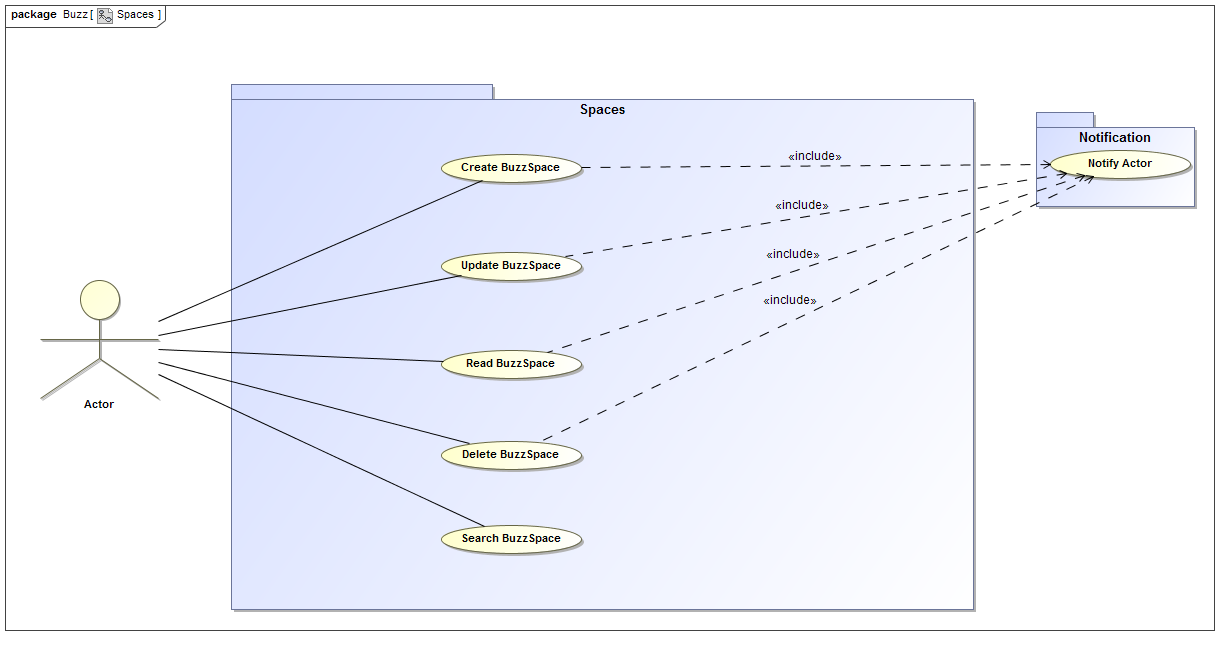
\includegraphics[width=\textwidth]{spacesUseCase}
	\subsection{Short description}
	\begin{description}
		
		\item[] 
			This section is for authentication relating to logging into the Buzz system and logging out of the system.
		
		\item[] Different actors:
		\begin{itemize}
			\item Administrator.
			\item User.   
		\end{itemize}
		
	\end{description}
	
	\subsection{Use case prioritization}
	\begin{description}
		\item[] Critical
		\begin{itemize}
			\item Login
			\item Logout
		\end{itemize}
	\end{description}
	
	\subsection{Use cases}
	\newpage
	\begin{longtable}{@{}|p{1.5cm}|p{2.2cm}|p{3cm}|p{3.5cm}|p{3.5cm}|@{}}
		\toprule
		\multicolumn{5}{|c|}{\textbf{Use cases for Space}}\\
		\hline
		\textbf{Actor} & \textbf{Use Case} & \textbf{Pre-condition} & \textbf{Post-Conditions} & \textbf{Description} \\ \midrule
		
		User Or Admin& 
		Login& 
		\begin{itemize}
			\item Buzz system must exist.
			\item User and administrator must be registered to use Buzz system.
		\end{itemize}& 
		\begin{itemize}
			\item User or admin will be logged into Buzz system.
		\end{itemize} & 
		User or admin logs into Buzz system. \\ \midrule
		
		User Or Admin& 
		Logout& 
		\begin{itemize}
			\item User and admin must be logged in.
		\end{itemize}& 
		\begin{itemize}
			\item User or admin will be logged out.
		\end{itemize} & 
		User or admin can log out of Buzz system \\ \bottomrule
		
		
		
	\end{longtable}
\end{document